\section{Transforming the Message Wave}

The message, given by \eqref{message} is shown below, between the bounds of 1V to -0.563V. However, as discussed previously, in order for the Variable Gain Amplifier to successfully encode the AM wave it needs the control voltage to vary between -1.34V and -1.21V. Thus, we need to transform the waveform. An Operational Amplifier, in this case an OPA207 from \textit{Texas Instruments}, can configured as an inverting summing amplifier to take care of both summing and attenuation of the signal. The configuration of the amplifier is shown below. Conducting Nodal Analysis of the the inverting amplifier, we see that the output will end up being
\begin{equation}\label{invertingAmp}
    V_{OUT} = -\frac{R2}{R1} * (V_1 + V_2)
\end{equation}

\begin{figure}[H]
    \centering
    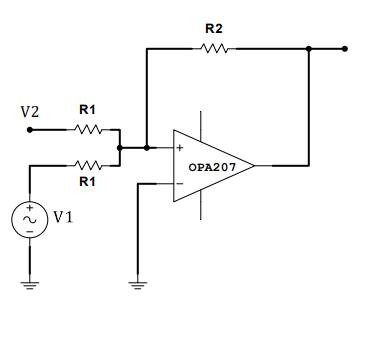
\includegraphics[width = 0.6\textwidth]{Images/OPA207.png}
    \caption{Inverting Summing Amplifier}
    \label{fig:Inverting Summing Amplifier}
\end{figure}

